\documentclass[11pt]{article}
\usepackage[T1]{fontenc}
\usepackage{lmodern}
\usepackage{parskip}
\usepackage[colorlinks=true,urlcolor=blue,linkcolor=black,citecolor=black]{hyperref}
\usepackage{graphicx}
\usepackage{amsmath}
\usepackage[utf8]{inputenc}
\usepackage[spanish]{babel}
\usepackage{fancyhdr}
\usepackage{csquotes}
\usepackage{lastpage}
\usepackage{array}
\usepackage{listings}
\usepackage{color}
\definecolor{dkgreen}{rgb}{0,0.6,0}
\definecolor{gray}{rgb}{0.5,0.5,0.5}
\definecolor{mauve}{rgb}{0.58,0,0.82}
\usepackage[affil-it]{authblk}
\usepackage[activate={true,nocompatibility},final,tracking=true,kerning=true,spacing=true,factor=1100,stretch=10,shrink=10]{microtype}
\usepackage[hmargin=2cm,top=4cm,headheight=65pt,footskip=65pt]{geometry}
\usepackage{hyperref}
\usepackage{graphicx}
\usepackage{float}
\usepackage{tabularx}
\graphicspath{ {./screenshots/} }

% Documento
\begin{document}

\begin{titlepage}
 \begin{center}
        \vspace*{1cm}
            
        \Huge
        \textbf{Prácticas de Laboratorio}
            
        \vspace{0.5cm}
        \LARGE
        Informática Forense y Auditoría
            
        \vspace{1.5cm}
            
        \textbf{Hugo Fonseca Díaz}\\
        UO258318\\
        \href{mailto:uo258318@uniovi.es}{uo258318@uniovi.es}
            
        \vfill
            
        Convocatoria Junio-Julio 2021.
            
        \vspace{0.8cm}
            
        
\includegraphics[width=0.3\textwidth]{other/uniovi_logo.jpg}
            
        \Large
        Escuela de Ingeniería Informática\\
        Universidad de Oviedo\\
        España\\
        28 de junio de 2021
            
    \end{center}
\end{titlepage}

\newpage

\tableofcontents

\newpage

% Introducción
\section{Introducción}
Los ejercicios de este documento se han realizado en una máquina cuyas características se muestran en la siguiente captura.

\begin{figure}[H]
  \caption{Sistema del alumno Hugo Fonseca Díaz.}
  \centering
    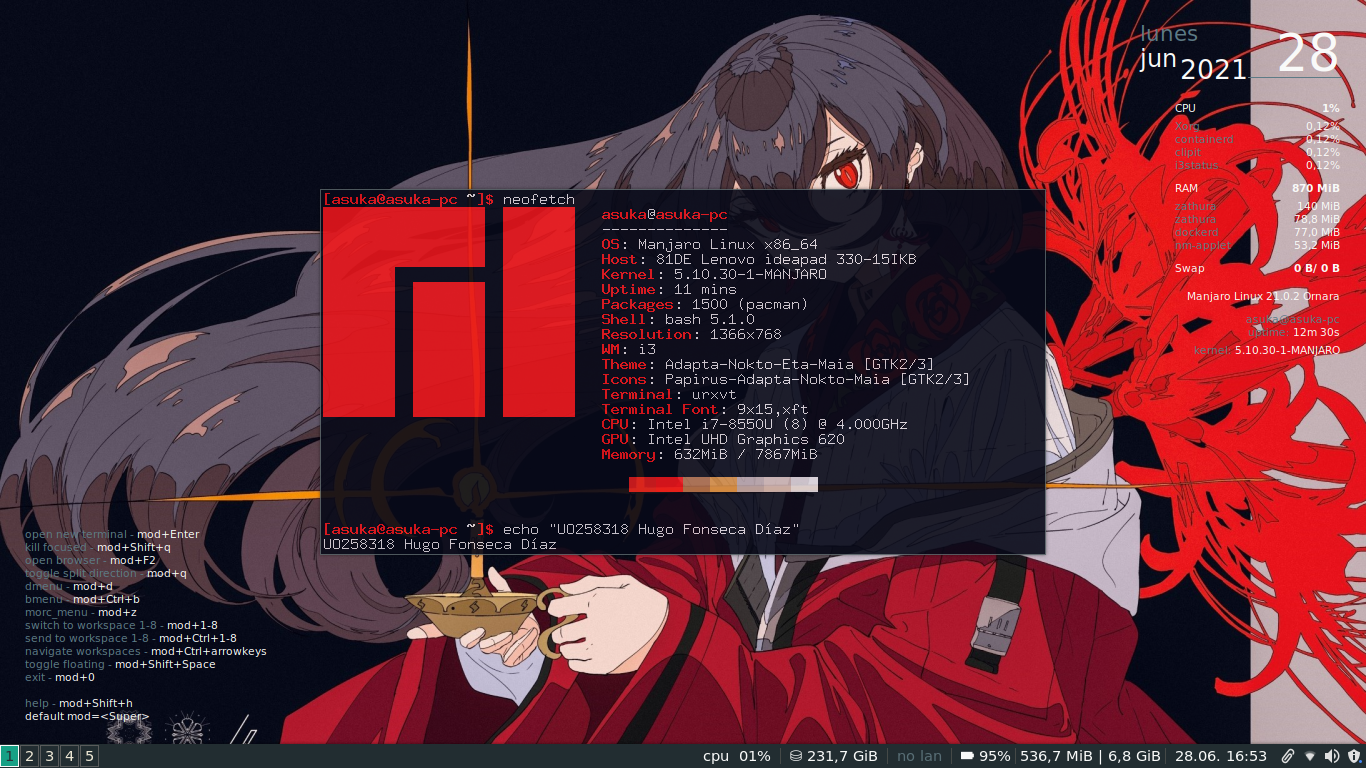
\includegraphics[scale=0.4, trim={0 1cm 0 0}, clip]{other/sistema_hugo.png}
\end{figure}

Las máquinas virtuales utilizadas pueden verse en la siguiente imagen.

\begin{figure}[H]
  \caption{Máquinas virtuales.}
  \centering
    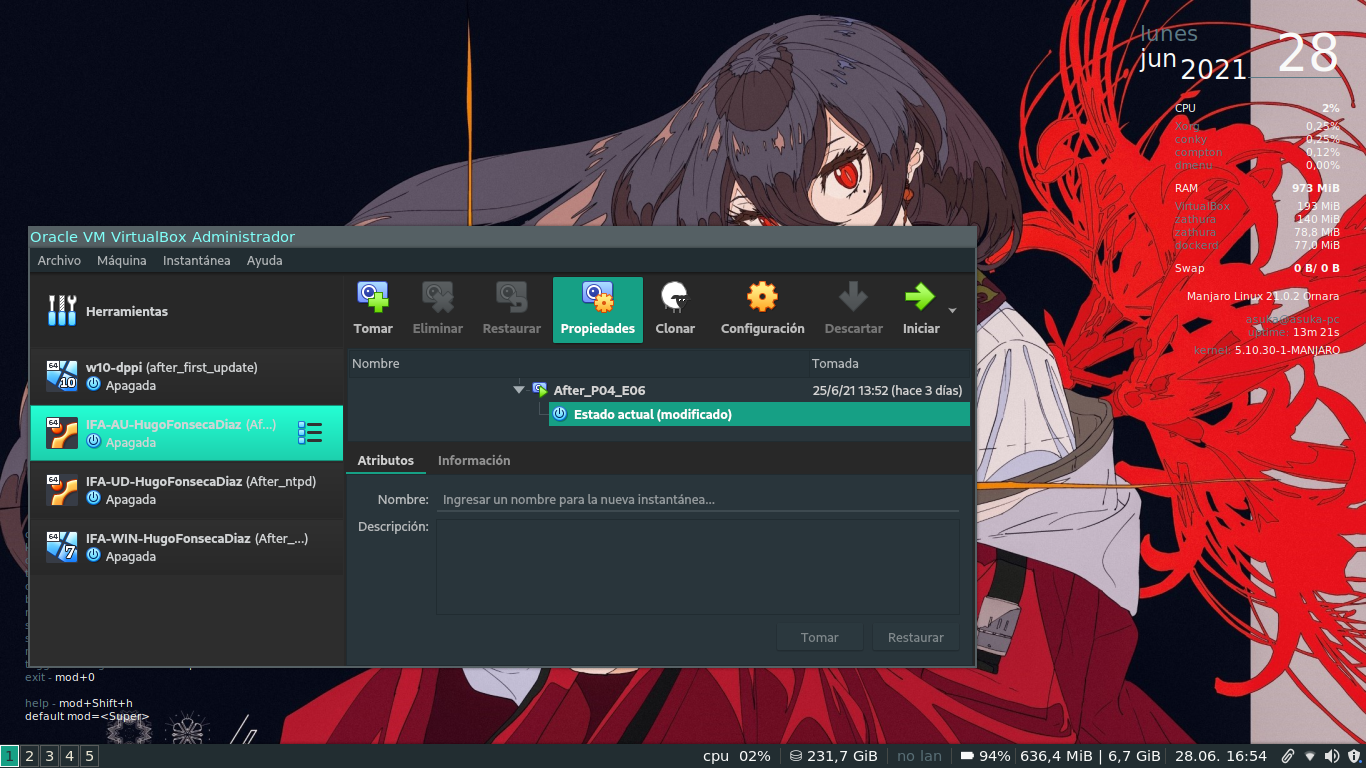
\includegraphics[scale=0.4, trim={0 1cm 0 0}, clip]{other/maquinas_virtuales_hugo.png}
\end{figure}

% Práctica 02
\section{Práctica 02}

\subsection{Ejercicio 27}
Se descomprime el archivo con el comando \verb|tar| y las flags \textit{xvzf}, siendo \textit{x} una indicación de que se quiere extraer los contenidos del archivo comprimido, \textit{v} para que lo haga de manera verbosa, \textit{z} para indicarle al comando que el archivo es un zip y \textit{f} para pasarle el fichero que se desea extraer al comando.

\begin{figure}[H]
    \caption{Ejercicio 27: \textit{tar -xvzf}.}
  \centering
  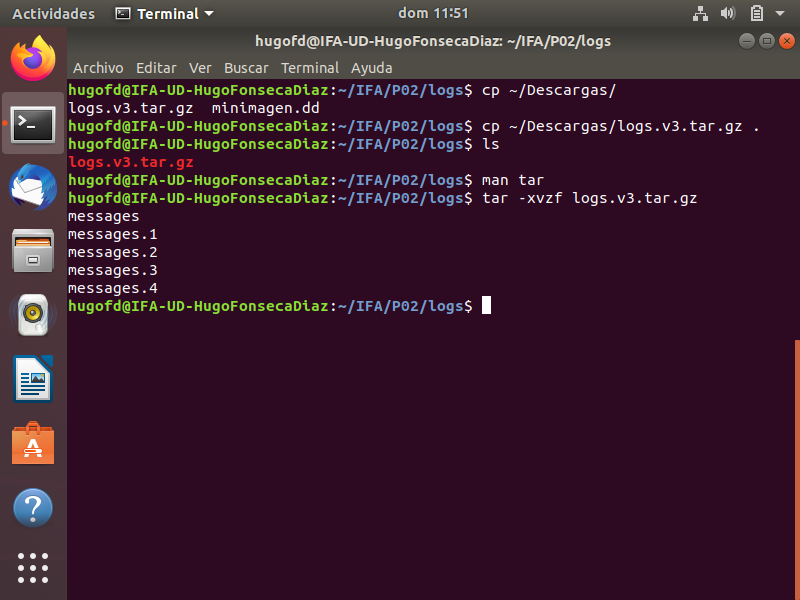
\includegraphics[scale=0.7, trim={0 7cm 0 0}, clip]{p02/e27-1.png}
\end{figure}

Una vez descomprimidos los ficheros de texto, se procede a utilizar tres nuevas herramientas. Se usa \verb|tac| para concatenar ficheros de forma inversa (es el comando \verb|cat| invertido), el lenguaje de programación AWK para procesar texto y el comando \verb|uniq| para omitir líneas repetidas.

\begin{figure}[H]
    \caption{Ejercicio 27: \textit{tac, AWK y uniq}.}
  \centering
  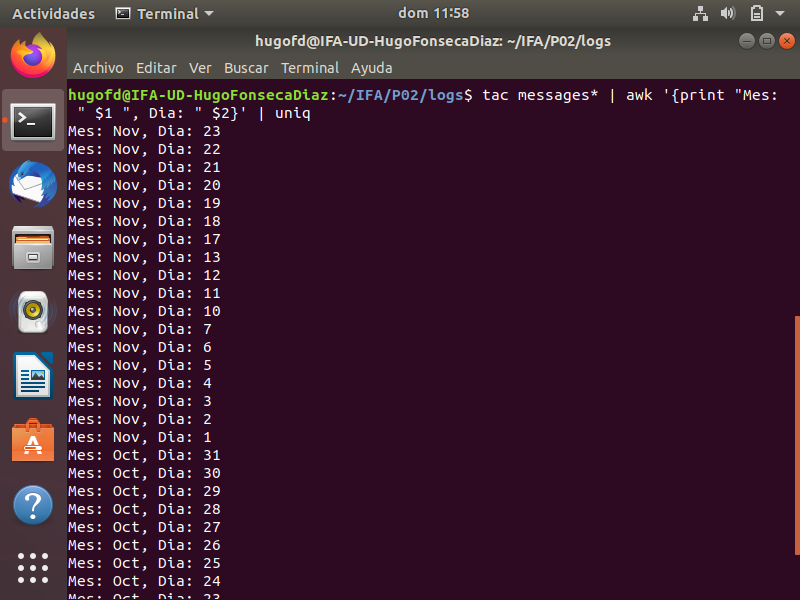
\includegraphics[scale=0.7]{p02/e27-2.png}
\end{figure}

\subsection{Ejercicio 31}
Se crea el caso en Autopsy con los datos solicitados.

\begin{figure}[H]
    \caption{Ejercicio 31: Creación del caso}
  \centering
  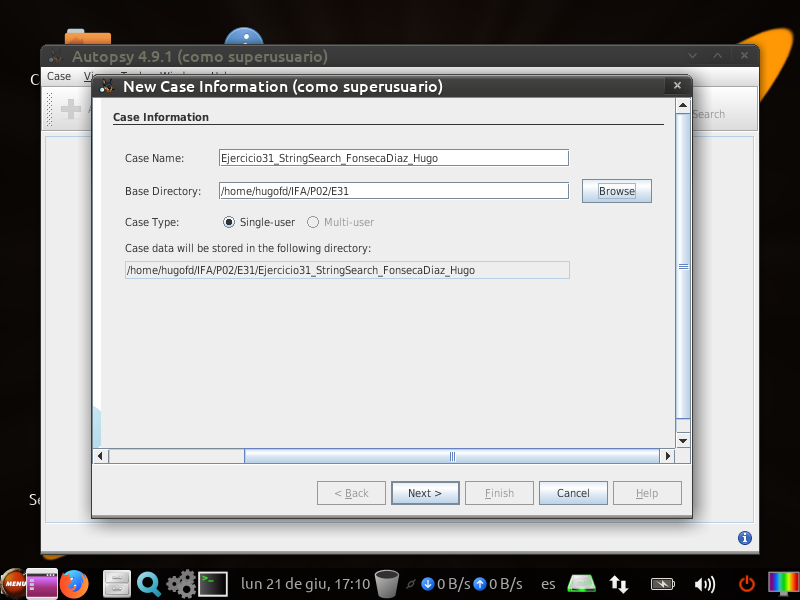
\includegraphics[scale=0.7]{p02/e31-1.png}
\end{figure}

\begin{figure}[H]
    \caption{Ejercicio 31: Selección de la imagen a analizar}
  \centering
  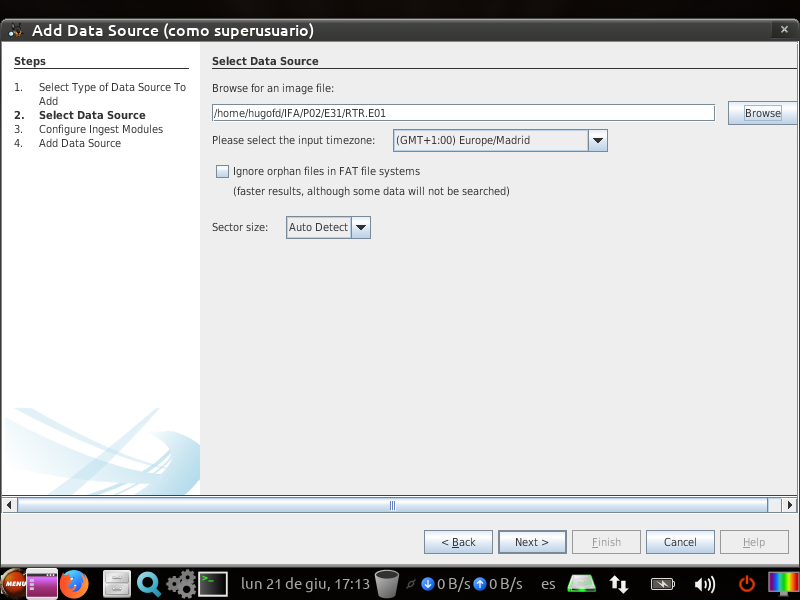
\includegraphics[scale=0.7]{p02/e31-2.png}
\end{figure}

Se seleccionan los módulos y se configura el módulo de búsqueda de palabras clave.

\begin{figure}[H]
    \caption{Ejercicio 31: Palabras clave}
  \centering
  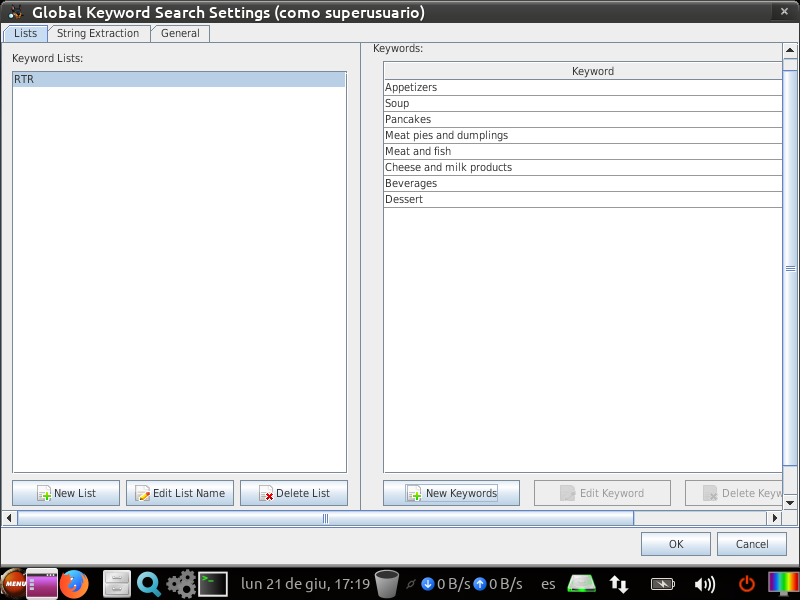
\includegraphics[scale=0.7]{p02/e31-3.png}
\end{figure}

\begin{figure}[H]
    \caption{Ejercicio 31: Módulos seleccionados}
  \centering
  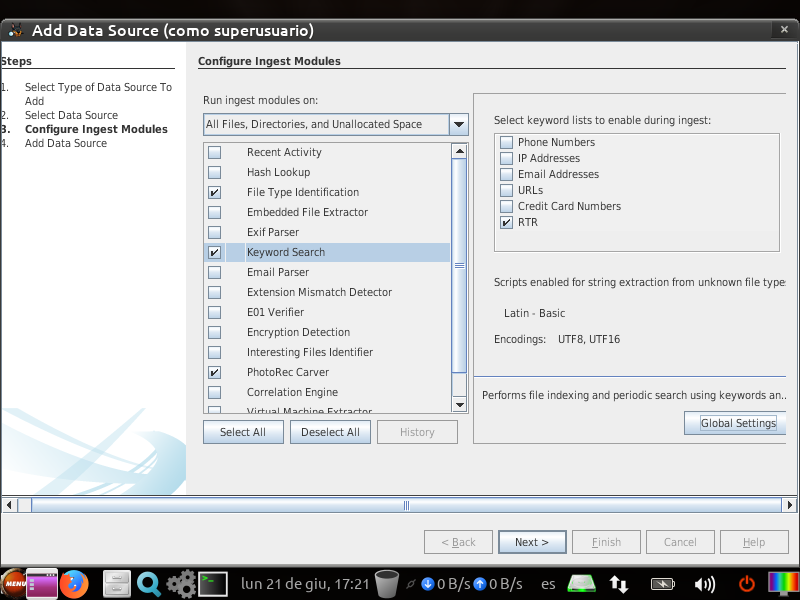
\includegraphics[scale=0.7]{p02/e31-4.png}
\end{figure}

\begin{figure}[H]
    \caption{Ejercicio 31: Configuración de los lenguajes de la búsqueda}
  \centering
  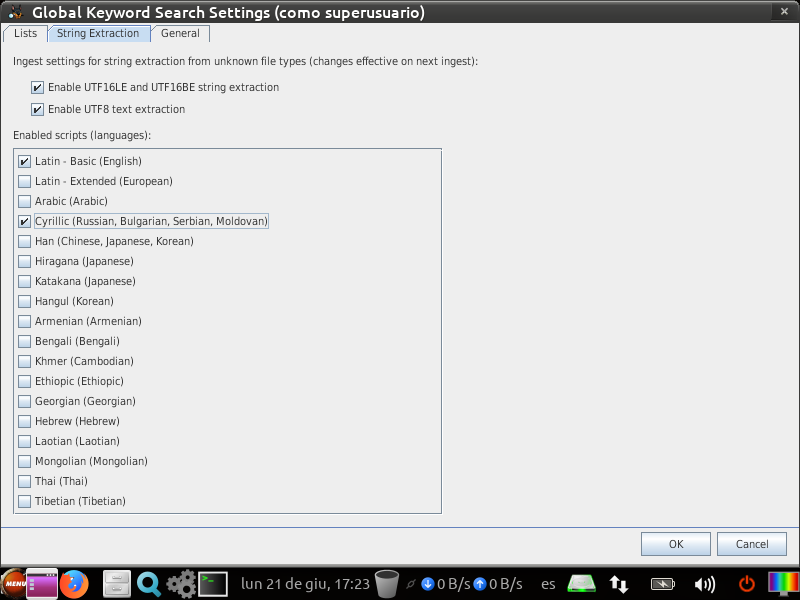
\includegraphics[scale=0.7]{p02/e31-5.png}
\end{figure}

Una vez finalizado el análisis, se pueden observar los ficheros encontrados.

\begin{figure}[H]
    \caption{Ejercicio 31: Resultados del análisis}
  \centering
  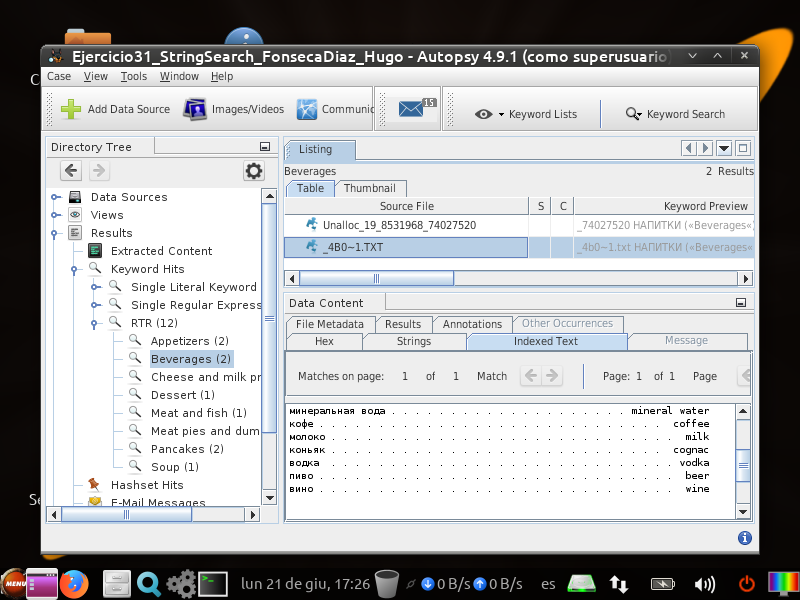
\includegraphics[scale=0.7]{p02/e31-6.png}
\end{figure}

Se reconstruye el menú del restaurante, creado inicialmente el 3 de noviembre de 2004.

\begin{figure}[H]
    \caption{Ejercicio 31: Menú reconstruido}
  \centering
  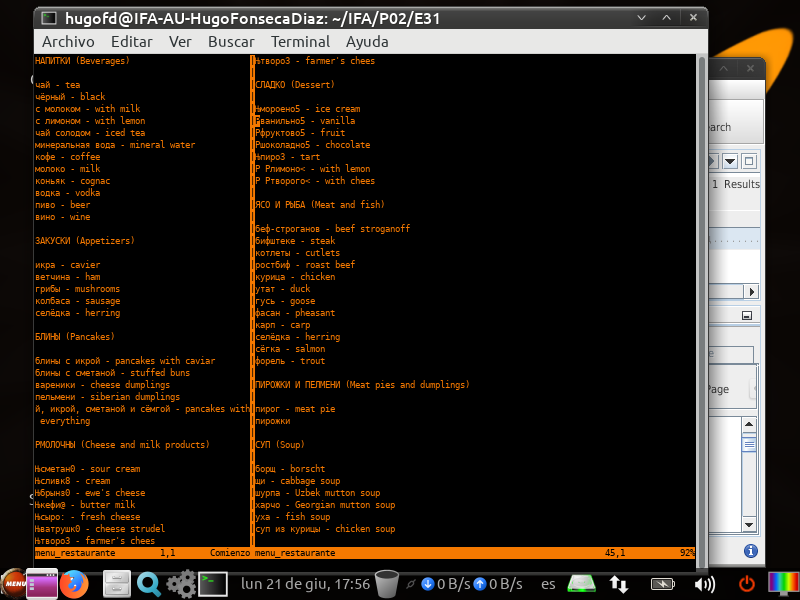
\includegraphics[scale=0.7]{p02/e31-7.png}
\end{figure}



% Práctica 03
\section{Práctica 03}

\subsection{Ejercicio 8}
Se crea el caso en Autopsy con los datos solicitados.

\begin{figure}[H]
    \caption{Ejercicio 8: Creación del caso}
    \centering
    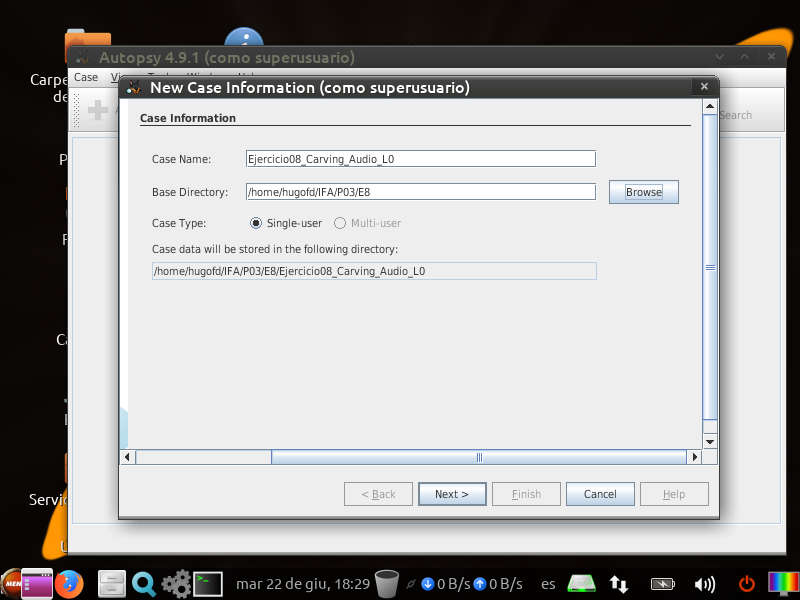
\includegraphics[scale=0.7]{p03/e8-1.png}
\end{figure}

\begin{figure}[H]
    \caption{Ejercicio 8: Detalles del examinador}
    \centering
    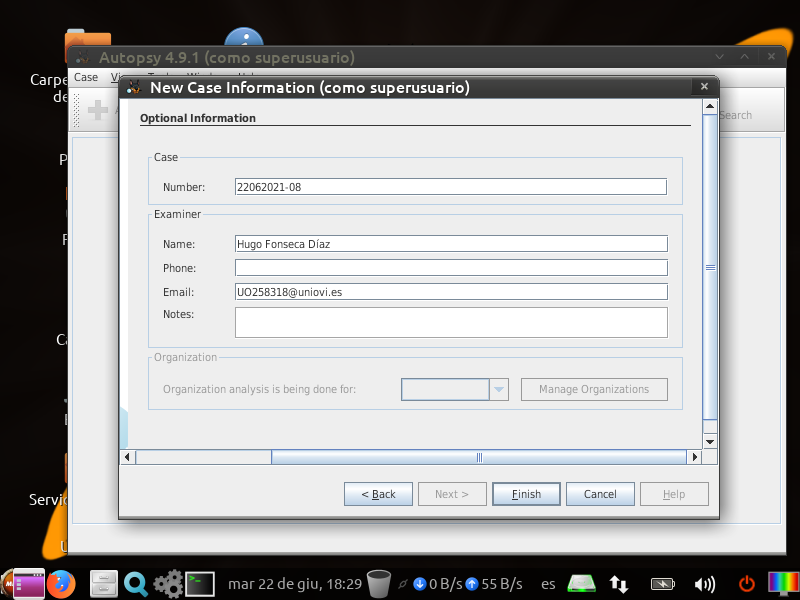
\includegraphics[scale=0.7]{p03/e8-2.png}
\end{figure}

Añadimos la imagen a analizar.

\begin{figure}[H]
    \caption{Ejercicio 8: Selección de la imagen}
    \centering
    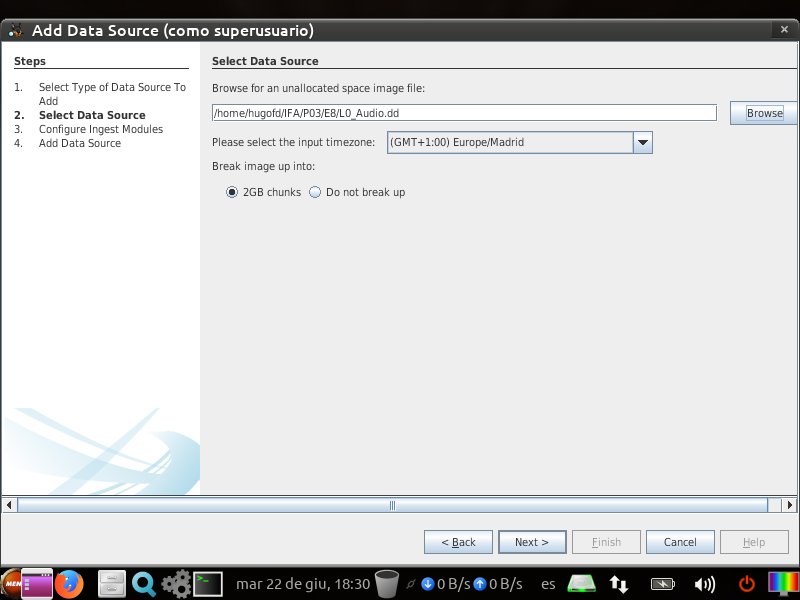
\includegraphics[scale=0.7]{p03/e8-3.png}
\end{figure}

Se seleccionan los módulos de identificación de tipos de fichero, parseador de Exif y \textit{PhotoRec Carver}.

\begin{figure}[H]
    \caption{Ejercicio 8: Selección de módulos}
    \centering
    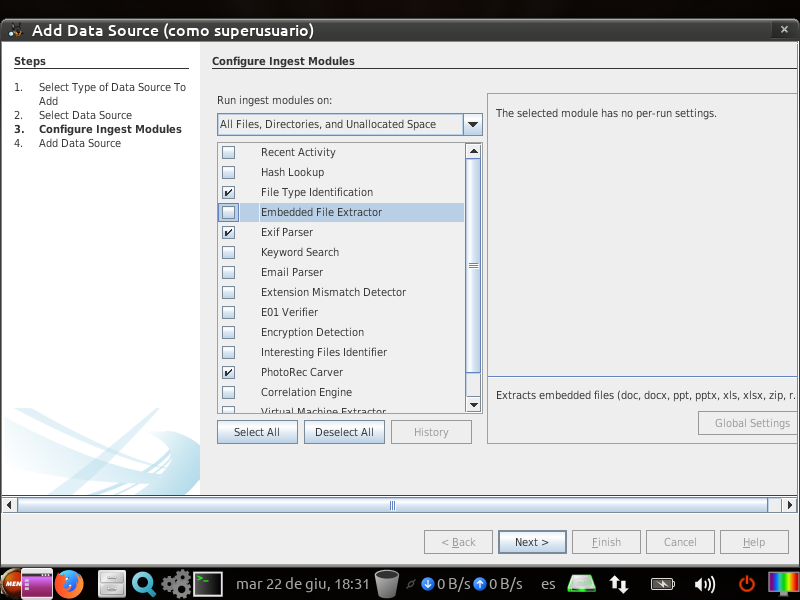
\includegraphics[scale=0.7]{p03/e8-4.png}
\end{figure}

Para rellenar la tabla se usarán los datos obtenidos al ejecutar el análisis de Autopsy y mediante el uso de la herramienta \textit{MediaInfo}.

\begin{figure}[H]
    \caption{Ejercicio 8: Resultados del análisis}
    \centering
    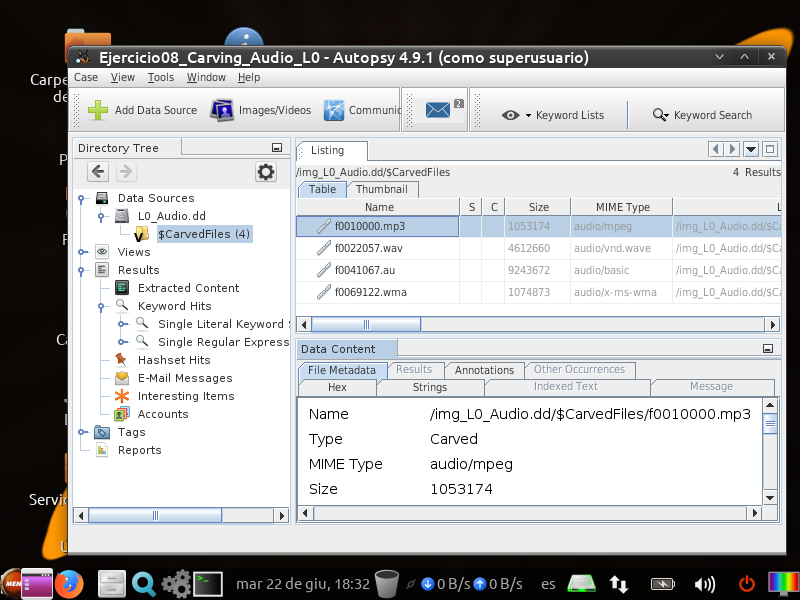
\includegraphics[scale=0.7]{p03/e8-5.png}
\end{figure}

\begin{figure}[H]
    \caption{Ejercicio 8: Herramienta \textit{MediaInfo}}
    \centering
    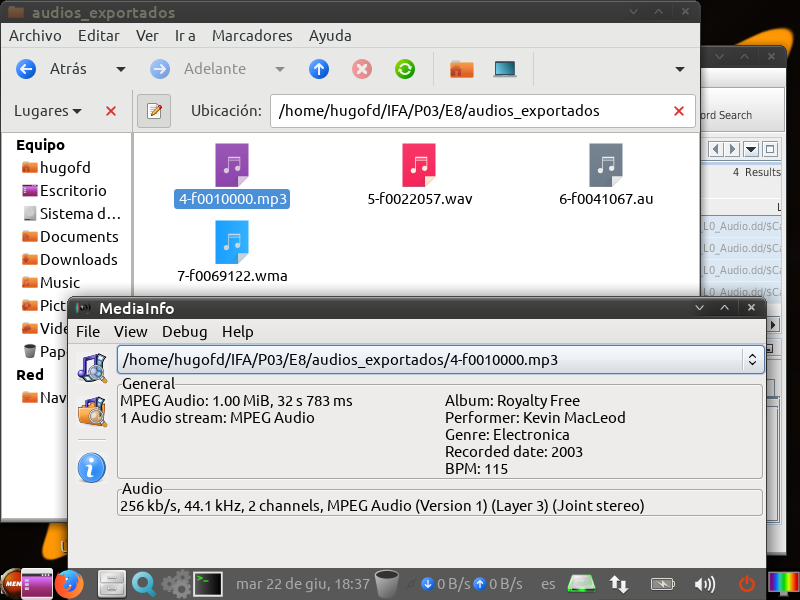
\includegraphics[scale=0.7]{p03/e8-6.png}
\end{figure}

\begin{table}[H]
    \centering
    \begin{tabular}{|p{2.5cm}|p{2cm}|c|p{1.5cm}|c|c|c|}
        \hline
        Nombre del fichero en Autopsy & Tamaño del fichero (en Bytes) & Tipo MIME & Autor & Género & Duración & Tasa de Muestreo \\
        \hline\hline
        f0010000.mp3 & 1053174 & audio/mpeg & Kevin McLeod & Electronica & 32s 783ms & 44.1kHz \\
        \hline
        f0022057.wav & 4612660 & audio/vnd.wave & - & - & 26s 148ms & 44.1kHz \\
        \hline
        f0041067.au & 9243672 & audio/basic & - & - & 3min 29s & 44.1kHz \\
        \hline
        f0069122.wma & 1074873 & audio/x-ms-wma & - & (80) & 1min 5s & 44.1kHz \\
        \hline
    \end{tabular}
\end{table}

\subsection{Ejercicio 13}
Se crea el caso en Autopsy con los datos solicitados.

\begin{figure}[H]
    \caption{Ejercicio 13: Creación del caso}
    \centering
    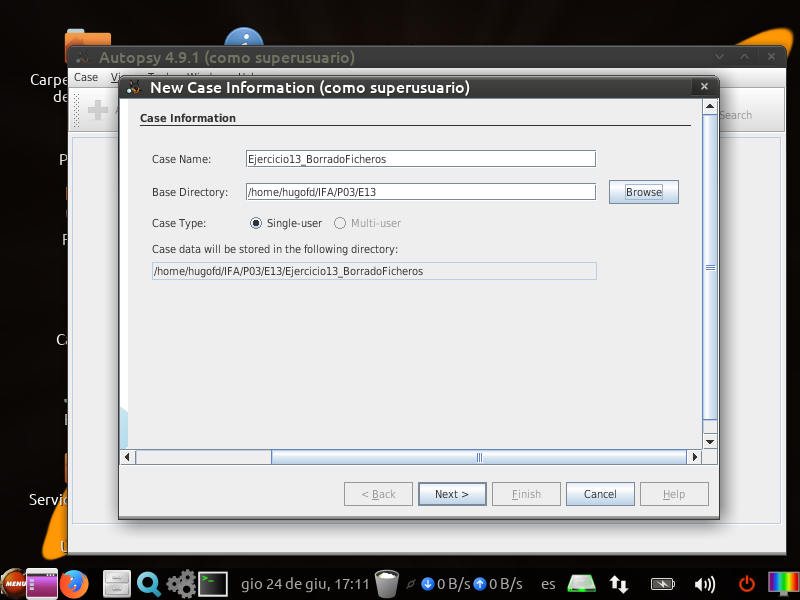
\includegraphics[scale=0.7]{p03/e13-1.png}
\end{figure}

\begin{figure}[H]
    \caption{Ejercicio 13: Detalles del examinador}
    \centering
    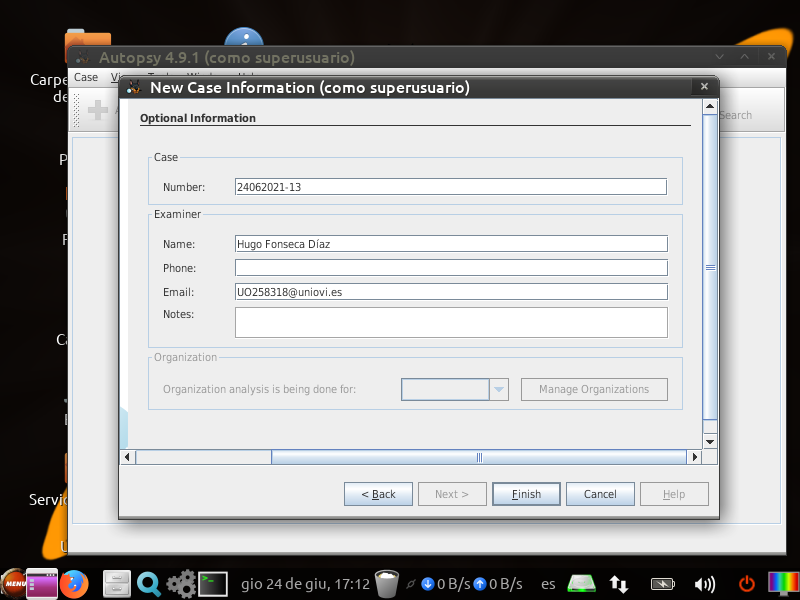
\includegraphics[scale=0.7]{p03/e13-2.png}
\end{figure}

Añadimos la imagen a analizar.

\begin{figure}[H]
    \caption{Ejercicio 13: Selección de la imagen}
    \centering
    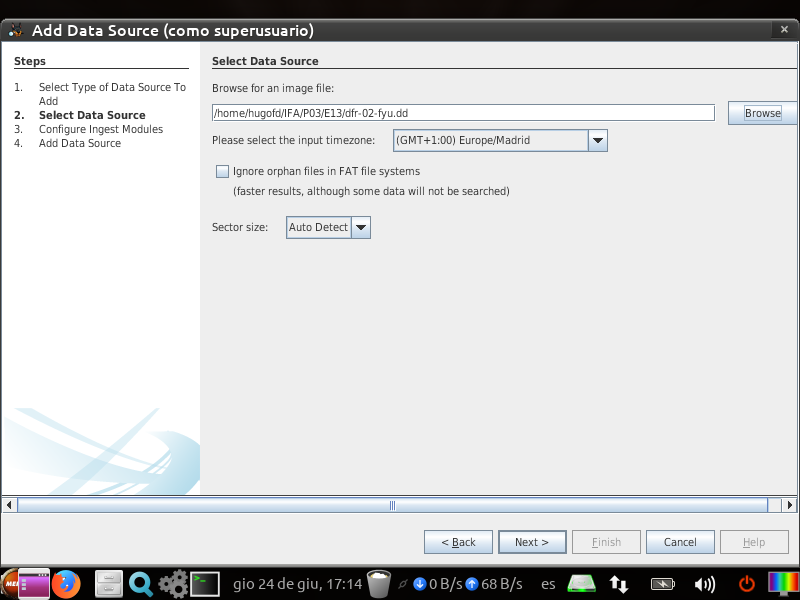
\includegraphics[scale=0.7]{p03/e13-3.png}
\end{figure}

Se seleccionan los módulos de identificación de tipos de fichero y \textit{PhotoRec Carver}.

\begin{figure}[H]
    \caption{Ejercicio 13: Selección de módulos}
    \centering
    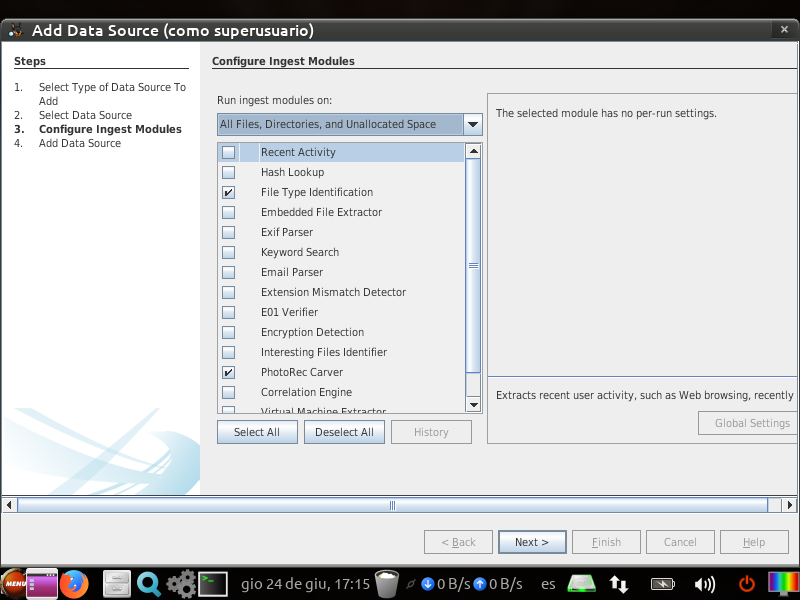
\includegraphics[scale=0.7]{p03/e13-4.png}
\end{figure}

Se obtienen los resultados del análisis con los que se responderán a las diferentes cuestiones del ejercicio.

\begin{figure}[H]
    \caption{Ejercicio 13: Resultados del análisis}
    \centering
    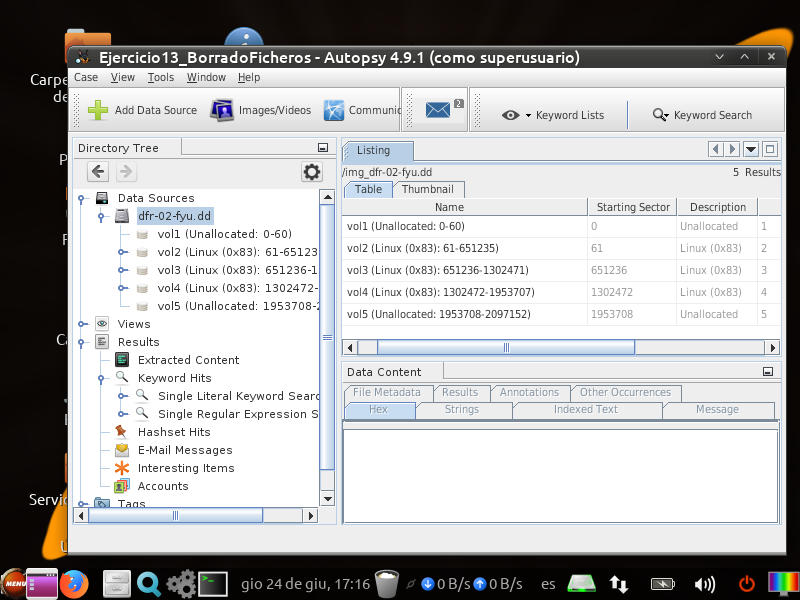
\includegraphics[scale=0.7]{p03/e13-5.png}
\end{figure}

a)

\begin{table}[H]
    \centering
    \begin{tabular}{|c|c|c|c|}
        \hline
        Número partición & Sector comienzo & Sector finalización & Tipo Sistema de Ficheros \\
        \hline\hline
        1 & 0 & 60 & Unallocated \\
        \hline
        2 & 61 & 651235 & Linux \\
        \hline
        3 & 651236 & 1302471 & Linux \\
        \hline
        4 & 1302472 & 1953707 & Linux \\
        \hline
        5 & 1953708 & 2097152 & Unallocated \\
        \hline
    \end{tabular}
\end{table}

b) Para responder a esta cuestión se observan los resultados de la pestaña 'Views'.

\begin{figure}[H]
    \caption{Ejercicio 13: Ficheros de texto plano}
    \centering
    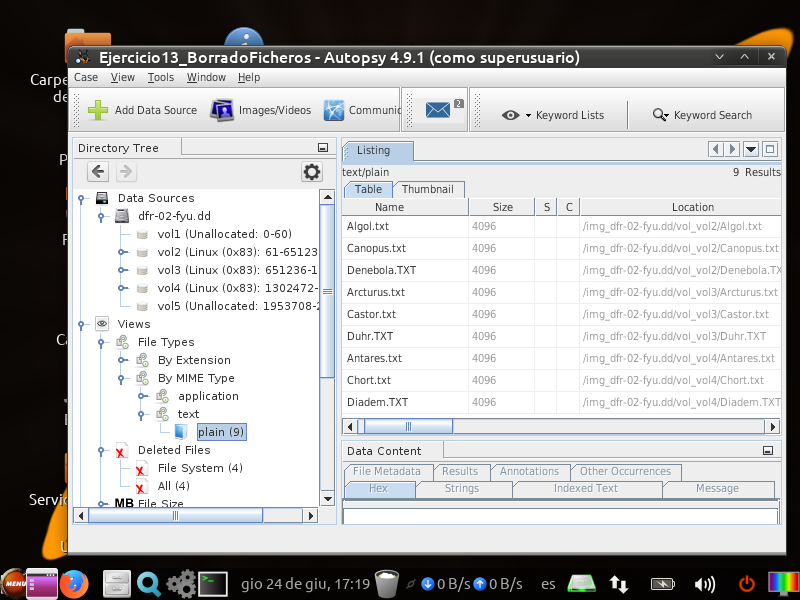
\includegraphics[scale=0.7]{p03/e13-6.png}
\end{figure}

Se puede ver que hay 9 ficheros de texto plano. Hay 4 ficheros adicionales borrados, uno llamado OrphanFiles, el cual es autogenerado por Autopsy, y tres ficheros con extensión txt pero cuyos tipos MIME no son texto plano.

c) Para rellenar esta tabla se miran los metadatos que muestra Autopsy de cada archivo borrado.

\begin{figure}[H]
    \caption{Ejercicio 13: Metadatos de los ficheros borrados}
    \centering
    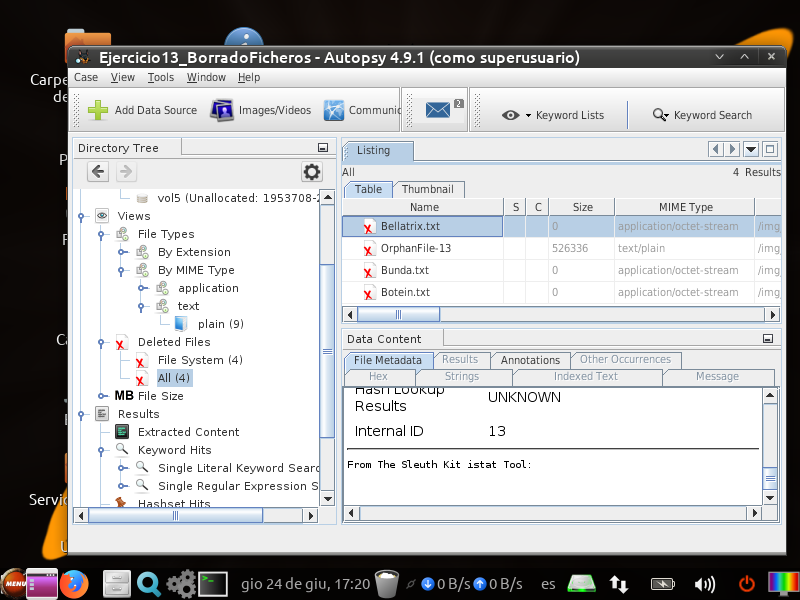
\includegraphics[scale=0.7]{p03/e13-7.png}
\end{figure}

Como se puede observar hay menos metadatos sobre los ficheros borrados que en el ejercicio anterior, por lo que habrá secciones de la tabla sin rellenar.

\begin{table}[H]
    \centering
    \begin{tabular}{|c|c|c|c|p{2cm}|p{2cm}|p{2cm}|}
        \hline
        Nombre & Tamaño & Partición & Sector relativo & Acceso (GMT) & Modificación (GMT) & Creación (GMT) \\
        \hline\hline
        Bellatrix.txt & 0 & vol 2 & - & - & - & - \\
        \hline
        Bunda.txt & 0 & vol 3 & - & 1999/01/02 08:04:00 & 2011/10/16 18:52:31 & 2011/10/16 18:52:31 \\
        \hline
        Botein.txt & 0 & vol 4 & - & 1999/01/02 08:05:00 & 2011/10/16 18:52:31 & 2011/10/16 18:52:31 \\
        \hline
    \end{tabular}
\end{table}

d) Se muestran a continuación las líneas de tiempo de los tres ficheros borrados, en el filtro de la parte izquierda de la captura se observa el fichero actual.

\begin{figure}[H]
    \caption{Ejercicio 13: Línea temporal de \textit{Bellatrix.txt}}
    \centering
    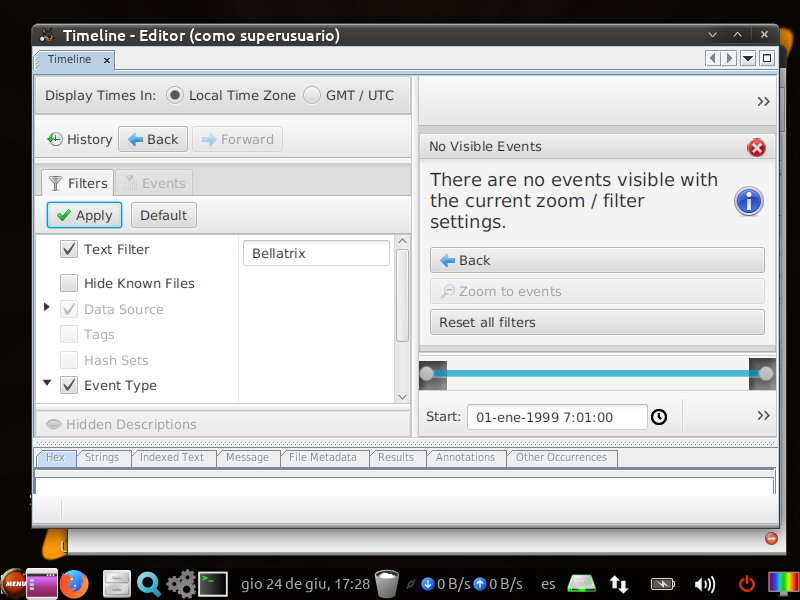
\includegraphics[scale=0.7]{p03/e13-8.png}
\end{figure}

Se observa que no hay datos para \textit{Bellatrix.txt}

\begin{figure}[H]
    \caption{Ejercicio 13: Línea temporal de \textit{Bunda.txt}}
    \centering
    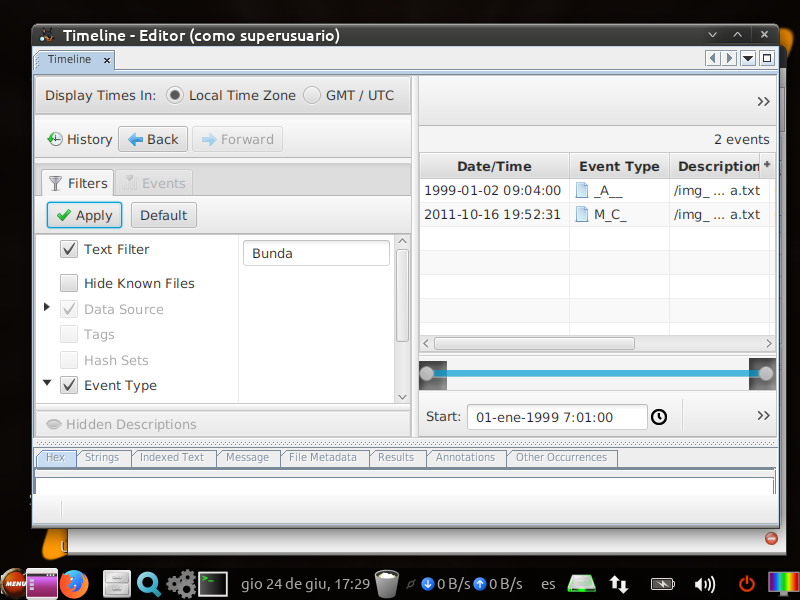
\includegraphics[scale=0.7]{p03/e13-9.png}
\end{figure}

\begin{figure}[H]
    \caption{Ejercicio 13: Línea temporal de \textit{Botein.txt}}
    \centering
    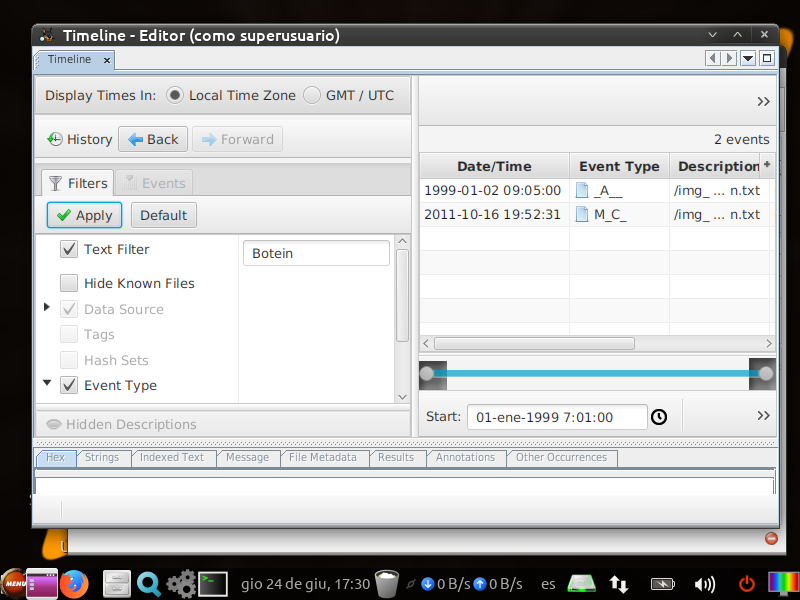
\includegraphics[scale=0.7]{p03/e13-10.png}
\end{figure}

Para \textit{Bunda.txt} y \textit{Botein.txt} sí que se recuperan datos.

\subsection{Ejercicio 14}
Se responde a continuación a las diferentes cuestiones planteadas por el ejercicio.

a) Se utiliza el comando \verb|mmls|, que lista las particiones con sus sectores de inicio y fin, entre otros datos.

\begin{figure}[H]
    \caption{Ejercicio 14: Salida del comando \textit{mmls}}
    \centering
    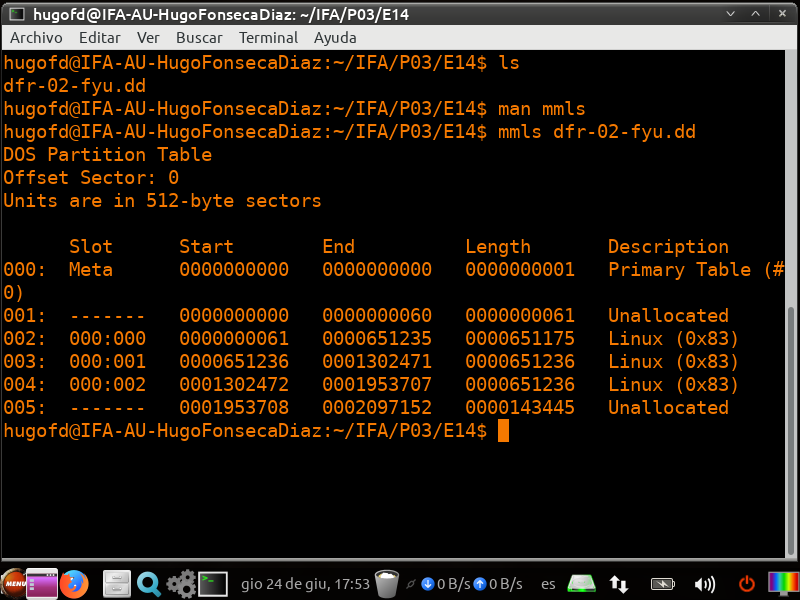
\includegraphics[scale=0.7]{p03/e14-1.png}
\end{figure}

b) Sí, la información es consistente entre ambas herramientas.

c) Se usa el comando \verb|fsstat|, con la flag \textit{t} para mostrar solo el tipo de partición y la flag \textit{o} para pasarle al comando el sector donde comienza la partición.

\begin{figure}[H]
    \caption{Ejercicio 14: Salida del comando \textit{fsstat} para las diferentes particiones}
    \centering
    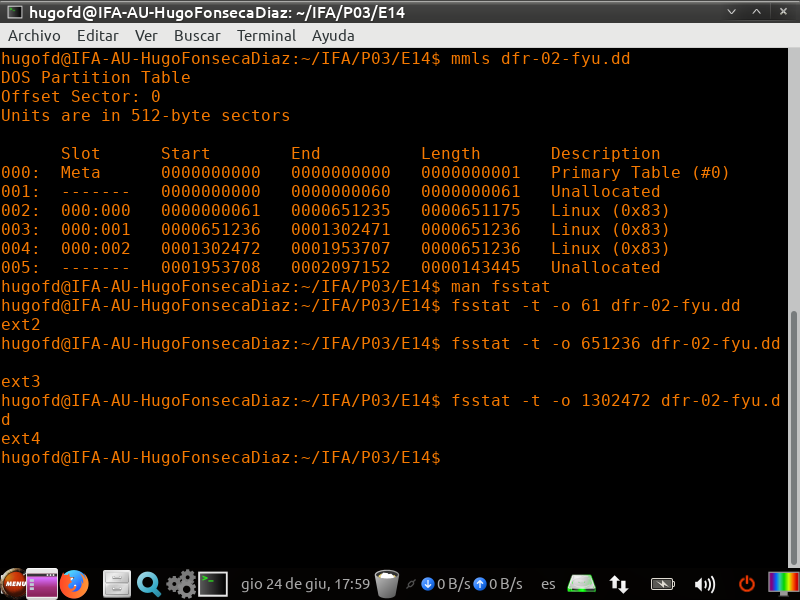
\includegraphics[scale=0.7]{p03/e14-2.png}
\end{figure}

d) Se utiliza el comando \verb|fls| que recibe como argumentos, entre otros, el comienzo del sector de la partición que se quiere analizar.

\begin{figure}[H]
    \caption{Ejercicio 14: Salida del comando \textit{fls} con las flags \textit{ro}}
    \centering
    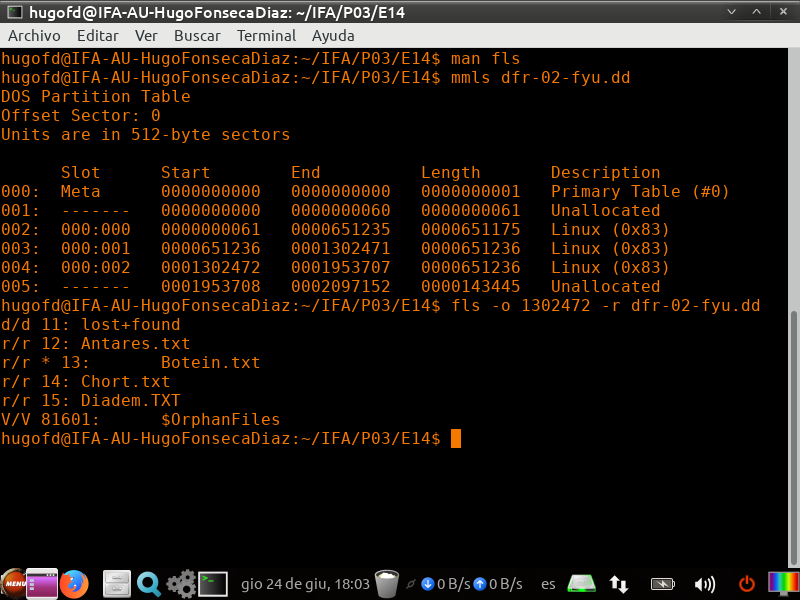
\includegraphics[scale=0.7]{p03/e14-3.png}
\end{figure}

e) Se usa ahora el comando \verb|fls| con las flags \textit{dFro}, \textit{d} muestra solo elementos borrados, \textit{F} muestra solo ficheros, \textit{r} es para que la búsqueda sea recursiva y \textit{o} para introducir el comienzo del sector de la partición.

\begin{figure}[H]
    \caption{Ejercicio 14: Salida del comando \textit{fls} con las flags \textit{dFro}}
    \centering
    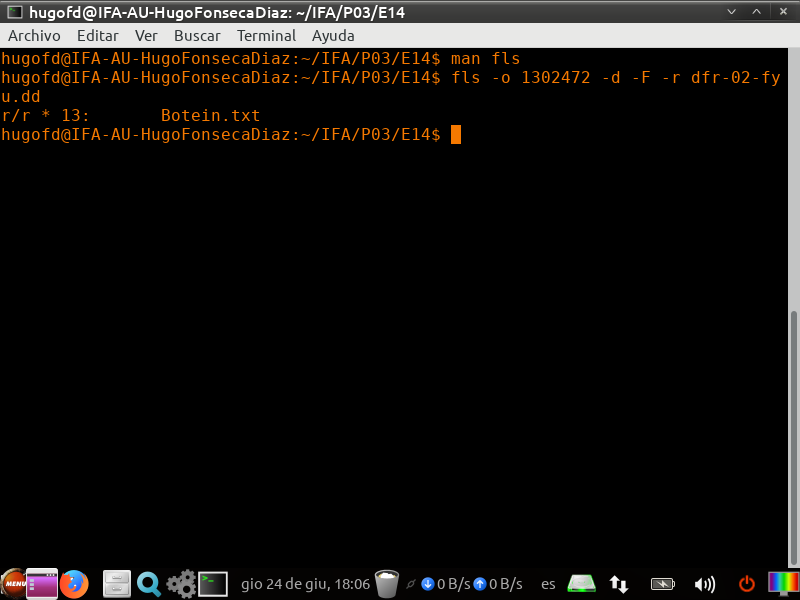
\includegraphics[scale=0.7]{p03/e14-4.png}
\end{figure}

f) Se utiliza el comando \verb|ffind| con las flags \textit{oa}, \textit{o} para introducir el comienzo del sector de la partición y \textit{a} para buscar todos los ficheros asociados. Se le pasa al comando el inodo del elemento que se está buscando, en este caso el 13.

\begin{figure}[H]
    \caption{Ejercicio 14: Salida del comando \textit{ffind}}
    \centering
    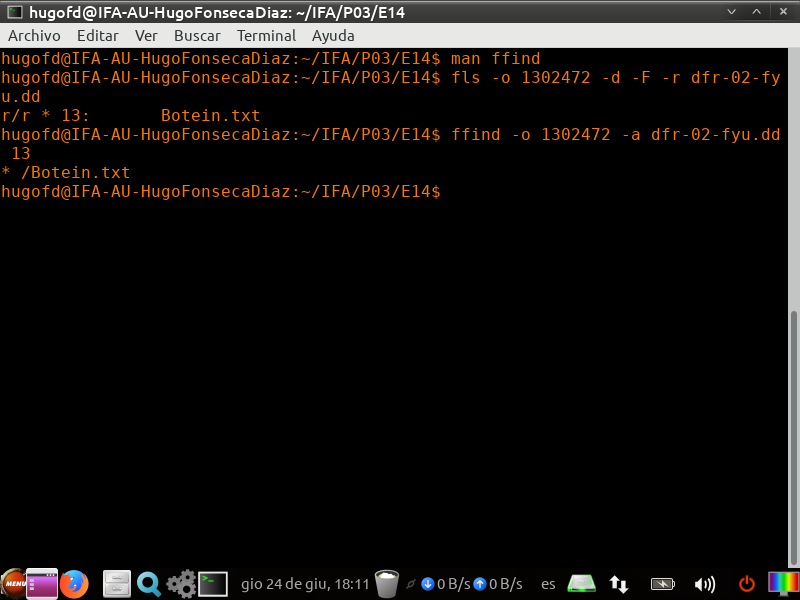
\includegraphics[scale=0.7]{p03/e14-5.png}
\end{figure}

g) Se usa el comando \verb|istat| pasandole como argumento el comienzo del sector de la partición y el inodo a buscar.

\begin{figure}[H]
    \caption{Ejercicio 14: Salida del comando \textit{istat} para el inodo 13}
    \centering
    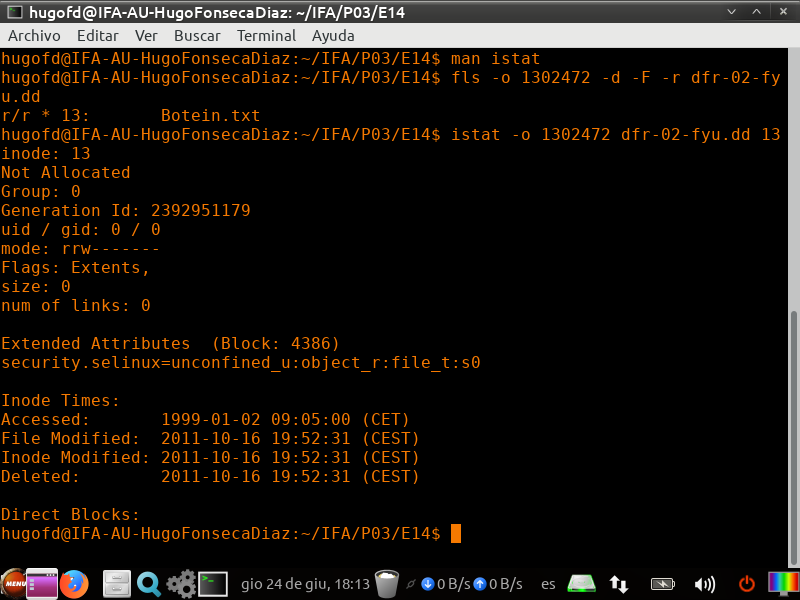
\includegraphics[scale=0.7]{p03/e14-6.png}
\end{figure}

h) Se usa el comando \verb|istat| con la flag \textit{f} y el argumento \textit{list}.

\begin{figure}[H]
    \caption{Ejercicio 14: Salida del comando \textit{istat -f list}}
    \centering
    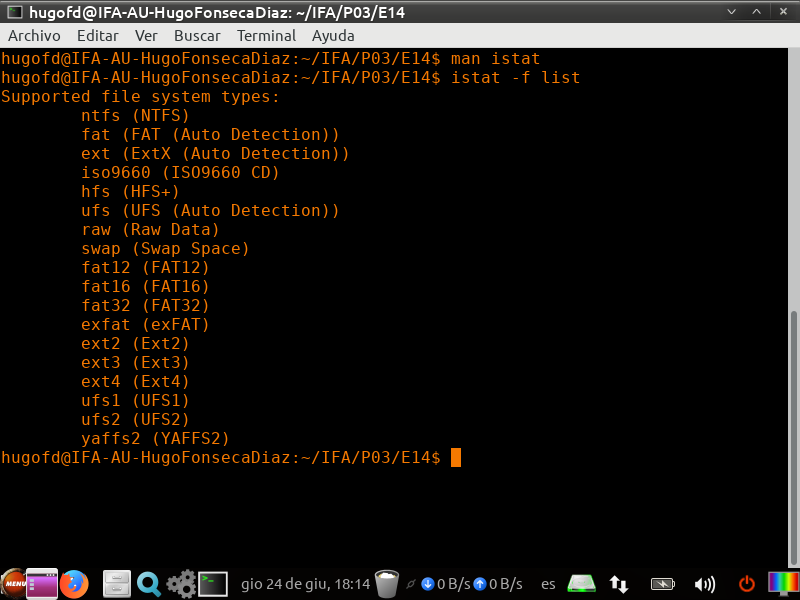
\includegraphics[scale=0.7]{p03/e14-7.png}
\end{figure}


\subsection{Ejercicio 19}

% Práctica 04
\section{Práctica 04}

% Práctica 05
\section{Práctica 05}


\end{document}




